% !TEX root = main.tex

\section{优化} % ch8, ch7
为了方便叙述,这里采用\href{http://cs229.stanford.edu/notes2019fall/cs229-notes-deep_learning.pdf}{Stanford CS229}的记号,矩阵微积分的推导主要参考:
\begin{itemize}
    \item Andrew Ng, Kian Katanforoosh, Anand Avati, \href{http://cs229.stanford.edu/notes2019fall/cs229-notes-deep_learning.pdf}{\emph{Stanford CS 229 Lecture Notes: Deep Learning}}
    \item Andrew Ng, Kian Katanforoosh, \href{http://cs229.stanford.edu/notes/cs229-notes-backprop.pdf}{\emph{Stanford CS 229 Lecture Notes: Backpropagation}}
    \item Kaare Brandt Petersen, Michael Syskind Pedersen, \href{https://www.math.uwaterloo.ca/~hwolkowi/matrixcookbook.pdf}{\emph{Matrix Cookbook}}
    \item \href{https://zhuanlan.zhihu.com/p/24709748}{矩阵求导术} - 长躯鬼侠的文章 - 知乎
    \item Daiwk,\href{https://daiwk.github.io/assets/matrix+vector+derivatives+for+machine+learning.pdf}{机器学习中的矩阵、向量求导}
\end{itemize}

\subsection{反向传播算法}
设输入特征为$x_1,x_2,\ldots$,即输入层。
$\smp{x}{i}$代表第$i$个训练样本,$\layer{z_j}{l}$代表第$l$层第$j$个神经元的输出,$\layer{a_j}{l}$代表激活后的输出,有
\[\begin{array}{rlrl}
x_1 &= \layer{a_1}{0} & & \\
x_2 &= \layer{a_2}{0} & & \\
\layer{z_1}{1}&=\layer{W_1}{1}^\T\vx+\layer{b_1}{1} &
\layer{a_1}{1}&=g(\layer{z_1}{1})\\
\layer{z_1}{2}&=\layer{W_1}{2}^\T\layer{\va}{1}+\layer{b_1}{2} &
\layer{a_1}{2}&=g(\layer{z_1}{2})
\end{array}\]
其中$W$是参数矩阵,$W_1$代表其中的第1行,激活后的输出为
\[\layer{\va}{1}=\bmat{
    \layer{a_1}{1}\\
    \layer{a_2}{1}\\
    \vdots
}\]

用矩阵的形式写,有
\[\underbrace{
\begin{bmatrix}
    \layer{z_1}{1}\\
    \layer{z_2}{1}\\
    \vdots\\
    \layer{z_m}{1}
\end{bmatrix}}_{\layer{\vz}{1}\in\rr^{m\times 1}}
=\underbrace{
\begin{bmatrix}
    \text{---} & \layer{W_1}{1}^\T & \text{---}\\
    & \vdots & \\
    & \vdots & \\
    \text{---} & \layer{W_m}{1}^\T & \text{---}
\end{bmatrix}}_{\layer{W}{1}\in\rr^{m\times n}}
\underbrace{
\begin{bmatrix}
    x_1\\
    \vdots\\
    x_n
\end{bmatrix}
}_{\vx\in\rr^{n\times 1}}
+\underbrace{
\begin{bmatrix}
    \layer{b_1}{1}\\
    \layer{b_2}{1}\\
    \vdots\\
    \layer{b_m}{1}
\end{bmatrix}
}_{\layer{\vb}{1}\in\rr^{m\times 1}}\]

因此有三层神经网络(单隐含层)的前向传播
\[\begin{aligned}
    \layer{\vz}{1} &= \layer{W}{1}\smp{\vx}{i} + \layer{\vb}{1}\\
    \layer{\va}{1} &= h(\layer{\vz}{1})\\
    \layer{\vz}{2} &= \layer{W}{2}\layer{\va}{1} + \layer{\vb}{2}\\
    \hat{\vy}^{(i)} &=\layer{\va}{2} = g(\layer{\vz}{2})
\end{aligned}\]
其中真实结果$\vy^{(i)}$为独热码(one-hot encoding)。

考虑损失函数(loss)为交叉熵
\[\mL(\hat{\vy},\vy)=-\vy^\T\ln\hat{\vy}\]
且激活函数$h(\cdot)$为sigmoid函数,$g(\cdot)$为softmax函数。

接下来推导反向传播(backpropagation, BP)算法,利用链式法则求导数。
比如想得到隐含层的权重,则计算
\[\pd{\mL}{\layer{W}{2}}=\pd{\mL}{\layer{\va}{2}}\pd{\layer{\va}{2}}{\layer{\vz}{2}}\pd{\layer{\vz}{2}}{\layer{W}{2}}\]
注意上式并非良定,其中涉及到实值函数对向量求导,也涉及到向量对向量求导(雅可比矩阵),还有向量对矩阵求导。
\[\begin{aligned}
\pd{\mL}{\layer{\va}{2}}
&=\pd{}{\layer{\va}{2}}(-\vy^\T\ln \va^{[2]}) \qquad\mbox{实数对向量求导}\\
&=-\frac{\vy}{\layer{\va}{2}} \qquad\mbox{逐元素相除}
\end{aligned}\]

设$\vu=\exp(\layer{\vz}{2})$为逐元素指数,分两步计算
\[\begin{aligned}
\pd{\layer{\va}{2}}{\vu}
&=\pd{}{\vu}\softmax(\layer{\vz}{2})\\
&=\pd{}{\vu}\frac{\exp(\layer{\vz}{2})}{\vone^\T\exp(\layer{\vz}{2})}\\
&=\pd{}{\vu}\frac{\vu}{\vone^\T\vu}\\
&=\vu\pd{(1/\vone^\T\vu)}{\vu^\T}+\frac{1}{\vone^\T\vu}\pd{\vu}{\vu} \qquad\mbox{乘法法则}\\
&=-\frac{1}{(\vone^\T\vu)^2}\vu\vone^\T+\frac{1}{\vone^\T\vu}I\\
\pd{\vu}{\layer{\vz}{2}}
&=\pd{\exp(\layer{\vz}{2})}{\layer{\vz}{2}}\\
&=\diag(\exp(\layer{\vz}{2}))\\
&=\diag(\vu)
\end{aligned}\]

由雅可比矩阵的链式法则
\[\begin{aligned}
\pd{\layer{\va}{2}}{\layer{\vz}{2}}
&=\pd{\layer{\va}{2}}{\vu}\pd{\vu}{\layer{\vz}{2}}\\
&=\lrp{-\frac{1}{(\vone^\T\vu)^2}\vu\vone^\T+\frac{1}{\vone^\T\vu}I}\diag(\vu)\\
&=-\frac{1}{(\vone^\T\vu)^2}\vu\vu^\T+\frac{1}{\vone^\T\vu}\diag(\vu)\\
&=-\frac{\vu}{\vone^\T\vu}\lrp{\frac{\vu}{\vone^\T\vu}}^\T+\frac{1}{\vone^\T\vu}\diag(\vu)\\
&=-\layer{\va}{2}\layer{\va}{2}^\T+\diag(\layer{\va}{2})
\end{aligned}\]

进而
\[\begin{aligned}
\pd{\mL}{\layer{\vz}{2}}
&:=\layer{\delta}{2} \qquad\mbox{损失函数对未激活前$\vz$的导数}\\
&=\lrp{\pd{\layer{\va}{2}}{\layer{\vz}{2}}}^\T\pd{\mL}{\layer{\va}{2}}\\
&=-\lrp{-\layer{\va}{2}\layer{\va}{2}^\T+\diag(\layer{\va}{2})}^\T\lrp{\frac{\vy}{\layer{\va}{2}}}\\
&=\layer{\va}{2}\lrp{\layer{\va}{2}^\T\frac{\vy}{\layer{\va}{2}}}-\diag(\layer{\va}{2})\lrp{\frac{\vy}{\layer{\va}{2}}}\\
&=\layer{\va}{2}\vone^\T\vy-\vy\\
&=\layer{\va}{2}-\vy \qquad\mbox{独热码满足$\vone^\T\vy=1$}
\end{aligned}\]

之后可计算
\[\begin{array}{lll}
\pd{\mL}{\layer{W}{2}}&=\pd{\mL}{\layer{\vz}{2}}\pd{\layer{\vz}{2}}{\layer{W}{2}}
&=\layer{\delta}{2}\layer{\va}{1}^\T \qquad\mbox{线性变换求导法则}\\
\pd{\mL}{\layer{b}{2}}&=\pd{\mL}{\layer{\vz}{2}}\pd{\layer{\vz}{2}}{\layer{b}{2}}
&=\layer{\delta}{2}
\end{array}\]

再往前推一层
\[\begin{aligned}
\pd{\mL}{\layer{\va}{1}}
&=\layer{W}{2}^\T\layer{\delta}{2}\\
\pd{\mL}{\layer{\vz}{1}}
&:=\layer{\delta}{1}\\
&=\pd{\mL}{\layer{\va}{1}}\pd{\layer{\va}{1}}{\layer{\vz}{1}}\\
&=\pd{\mL}{\layer{\va}{1}}\odot h'(\layer{\vz}{1})\\
&=\lrp{\layer{W}{2}^\T\layer{\delta}{2}}\odot h(\layer{\vz}{1})\odot (\vone-h(\layer{\vz}{1}))\\
\pd{\mL}{\layer{W}{1}}&=\layer{\delta}{1}\vx^\T\\
\pd{\mL}{\layer{\vb}{1}}&=\layer{\delta}{1}\\
\pd{\mL}{\vx}&=\layer{W}{1}^\T\layer{\delta}{1}
\end{aligned}\]

总结来说,对于第$n_l$层,\textcolor{red}{
\[\layer{\delta}{n_l}=-(\vy-\layer{\va}{n_l})\odot g'(\layer{\vz}{n_l})=\layer{\tilde{\delta}}{n_l}\odot g'(\layer{\vz}{n_l})\]
}
对于第$l=n_l-1,n_l-2,\ldots,1$层,
\textcolor{red}{
\[\layer{\delta}{l}=\lrp{\layer{W}{l+1}^\T\layer{\delta}{l+1}}\odot h'(\layer{\vz}{l})=\layer{\tilde{\delta}}{l}\odot h'(\layer{\vz}{l})\]
}
则有权重和偏置的梯度\textcolor{red}{
\[\begin{aligned}
\nabla_{\layer{W}{l}}\mL(W,b)&=\layer{\delta}{l}\layer{\va}{l-1}^\T\\
\nabla_{\layer{b}{l}}\mL(W,b)&=\layer{\delta}{l}
\end{aligned}\]
}

\subsection{梯度下降}
\subsubsection{挑战}
神经网络优化的过程中主要存在以下这些挑战:
\begin{itemize}
    \item 病态(ill-conditioning)Hessian矩阵:小步长也会导致大损失(参见数值计算)
    \item 局部极小值
    \item 平台(plateau)和鞍点(saddle point)
    \item 悬崖和梯度爆炸:梯度裁剪(clipping)可解决
    \item 长期依赖:网络太深时会导致梯度消失或爆炸
\end{itemize}

\subsubsection{基本算法}
\begin{itemize}
    \item 批梯度下降
    \[\vtheta_{t+1}=\vtheta_t-\frac{\eta}{N}\sum_{n=1}^N\nabla\mL(\vy_n,\vf(\vx_n;\vtheta_t))\]
    \item 随机梯度下降(SGD)
    \[\vtheta_{t+1}=\vtheta_t-\eta\nabla\mL(\vy_n,\vf(\vx_n;\vtheta_t))\]
    \item 子批(minibatch)梯度下降
    \[\vtheta_{t+1}=\vtheta_t-\frac{\eta}{|S|}\sum_{(\vx_n,\vy_n)\in S}\nabla\mL(\vy_n,\vf(\vx_n;\vtheta_t))\]
\end{itemize}

添加Nesterov动量(momentum)项,使得梯度下降可以保持原来的方向,以减少震荡
\[\begin{cases}
    \vnu_{t+1}=\textcolor{red}{\gamma\vnu_t}-\eta\nabla\mL(\vtheta_t)\\
    \vtheta_{t+1}=\vtheta_t+\vnu_{t+1}
\end{cases}\]
通常$\gamma$取$0.9$。

\begin{figure}[H]
\centering
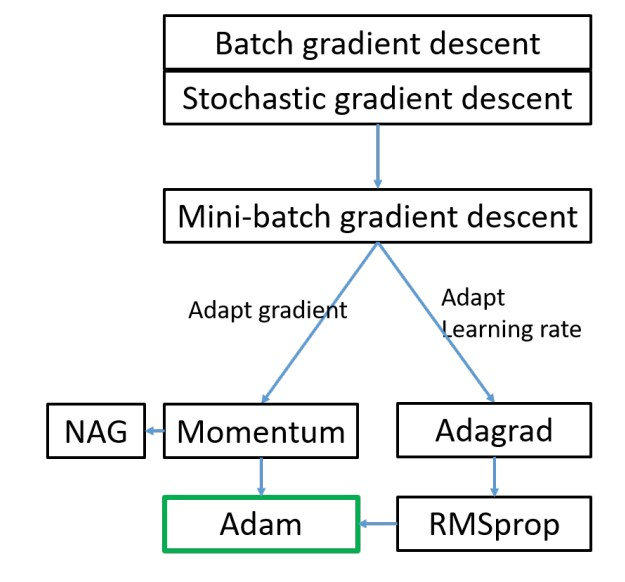
\includegraphics[width=0.5\linewidth]{fig/gd_catalog.jpg}
\caption{梯度下降算法分类}
\end{figure}